\newpage
\section{Funzionalità}
\label{sect:funz}
\rhead{Funzionalità}
Vengono ora presentate e spiegate nei minimi dettagli le funzionalità offerte dal Framework:
\begin{itemize}[nosep]
\item \textbf{Offuscamento dei dati}
\item \textbf{Automatizzazione dei test}  
\item \textbf{Offuscamento dei dati e automatizzazione dei test} 
\end{itemize}
\smallskip
\noindent Per ogni funzionalità verrà presentata l'architettura della soluzione ponendo particolare attenzione a:
\begin{itemize}[nosep]
\item[-]  ciò che permette di fare
\item[-]  parametri di esecuzione (obbligatori e facoltativi)
\item[-]  informazioni necessarie al funzionamento (ottenute dai file di configurazione e dai file di input)
\item[-] file prodotti in output
\end{itemize}
\bigskip
\noindent  Nel capitolo non verranno quindi analizzati i dettagli implementativi, che saranno oggetto invece dell'analisi nel capitolo successivo (Capitolo \ref{cap:dettagli}).

\newpage

\subsection{Offuscamento dei dati}
La funzionalità 'Offuscamento dei dati' si occupa dell'offuscamento dei dati rispondendo al requisito funzionale \emph{Fu.1}. Specificatamente la funzionalità permette di offuscare una o più colonne del file in input (ognuna delle quali appartenente ad un certo dominio) applicando una determinata tecnica di offuscamento per un numero specifico di iterazioni. 

\subsection*{Architettura della soluzione}
\begin{figure}[H]
	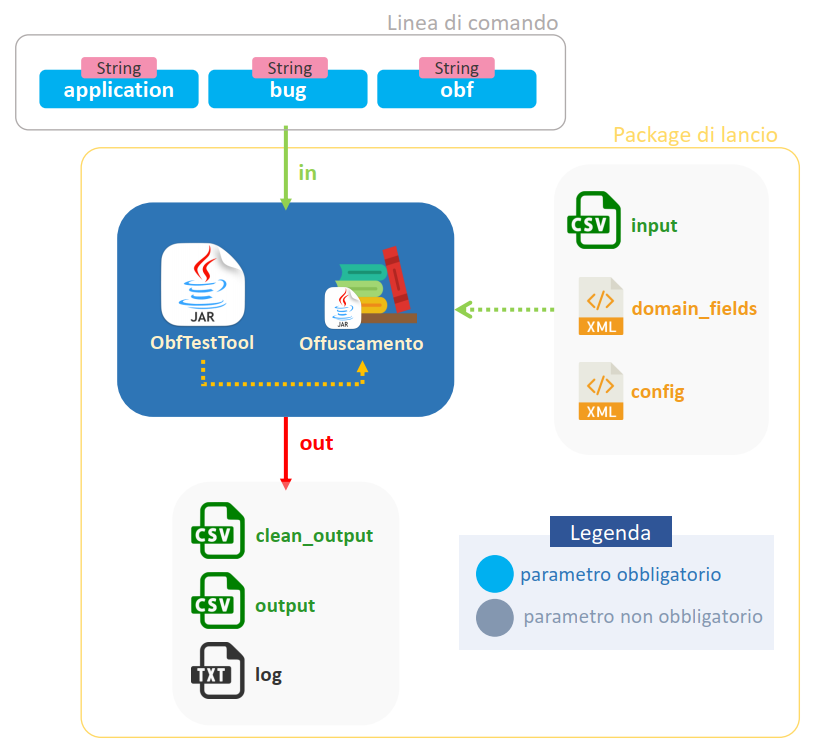
\includegraphics[scale=0.65]{obfuscation.architettura}
	\centering
	\caption{Architettura della soluzione}%\footnote{Immagine realizzata da A. Belisario}
    \label{fig:obfarch}
\end{figure}
Come illustrato in Figura \ref{fig:obfarch}, il tool, nell'eseguire la funzionalità considerata, richiede obbligatoriamente alcuni parametri:
\begin{itemize} [nosep]
\item \textbf{\emph{@application}} id dell'applicazione \emph{[dominio: String]}
\item \textbf{\emph{@bug}} id del bug \emph{[dominio: String]}
\item \textbf{\emph{@obf}} id della funzione di offuscamento \emph{[dominio: String]}
\end{itemize}
\bigskip
\noindent Grazie ai parametri passati, lo strumento è in grado di leggere dal package di lancio (Sezione \ref{sub:strpackage}) alcune informazioni essenziali all'esecuzione della funzionalità:
\begin{itemize} [nosep]
\item [$\blacksquare$]\textbf{tuple da offuscare} \newline
Ottiene le tuple da offuscare leggendo il file di input posizionato nel package di lancio nel percorso src/\emph{@application}/\emph{@bug}/input.csv

\item  [$\blacksquare$] \textbf{tecnica di offuscamento, colonne da offuscare, numero di ripetizioni} \newline
Ottiene queste informazioni leggendo il file di configurazione posizionato nel percorso src/config.xml. In particolar modo, effettuando il parsing del file xml, è in grado di ottenere le informazioni della tecnica di offuscamento con id \emph{@obf} relativa al bug con id \emph{@bug} dell'applicazione con id \emph{@application}.

\item  [$\blacksquare$]\textbf{id del dominio delle colonne} \newline
Ottiene l'id del dominio di ogni colonna leggendo il file di configurazione posizionato nel percorso src/config.xml. In particolar modo, effettuando il parsing del file xml, è in grado di ottenere gli identificativi dall'attributo delle colonne relative al bug con id \emph{@bug} dell'applicazione con id \emph{@application}.

\item  [$\blacksquare$]\textbf{dominio delle colonne} \newline
Ottiene le informazioni relative al dominio delle colonne leggendo il file di configurazione dei domini posizionato nel percorso src/\emph{@application}/domain\_fields.xml. In particolar modo, effettuando il parsing del file xml è in grado di ottenere le informazione del dominio con un certo id, che ricava come spiegato nel punto precedente.
\end{itemize}
\bigskip
\noindent In Figura \ref{fig:letcon} viene riportato un esempio della lettura delle informazioni 'tecnica di offuscamento', 'colonne da offuscare' e 'numero di ripetizioni'.

\begin{figure}[H]
	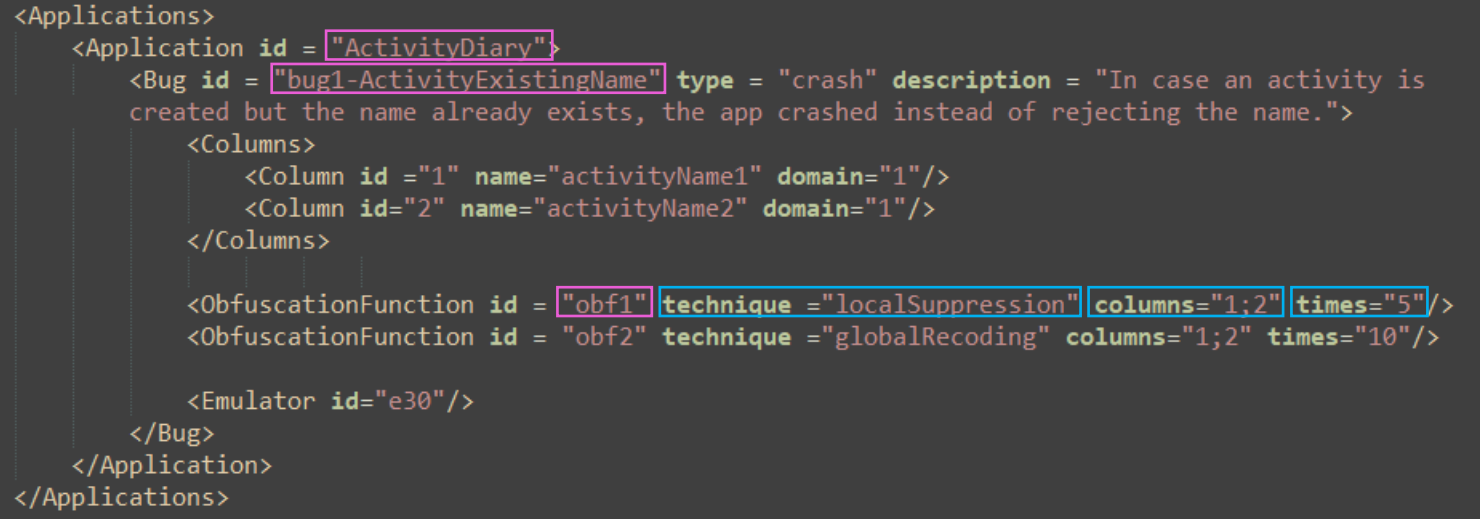
\includegraphics[scale=0.45]{lettura.config}
	\centering
	\caption{Esempio: lettura dal file di configurazione}
	\emph{Lettura di tecnica di offuscamento (technique), colonne da offuscare (columns) e numero di ripetizioni (times) per l'esecuzione della funzionalità con parametri in input @application="ActivityDiary", @bug="bug1-ActivityExistingName", @obf="obf1".}
    \label{fig:letcon}
\end{figure}
\smallskip
\noindent A questo punto il tool è in possesso di tutte le informazioni necessarie ad eseguire la funzionalità e può offuscare le tuple utilizzando i metodi offerti dalla libreria di offuscamento. 
\bigskip  \newline 
\noindent L'esecuzione della funzionalità, nel caso in cui vada a buon fine, porta alla produzione dei seguenti file:

\begin{tcolorbox}[colback=white, colframe=lightgray]
	 
\includegraphics[height=1cm]{icona.clean} \newline
Il file \emph{clean\_output.csv} contiene semplicemente le tuple prodotte dall'offuscamento, precedute da un'intestazione composta dai nomi delle colonne. Il file 'pulito' può essere utilizzato, senza nessuna modifica, come file di input  per l'automazione dei test (funzionalità 'Automatizzazione dei test'). Il suo mantenimento in memoria è di fondamentale importanza in quanto non basterebbe rieseguire la funzionalità con gli stessi parametri per ottenere i medesimi valori offuscati, poichè alcune delle tecniche di offuscamento dipendono da un fattore randomico. In Figura \ref{fig:obf.clean.es} viene mostrato un esempio del file prodotto. 
\end{tcolorbox}

\begin{tcolorbox}[colback=white, colframe=lightgray]
	 
\includegraphics[height=1cm]{icona.output} \newline
Il file \emph{output.csv} può essere considerato il file riepilogativo dell'esecuzione della funzionalità in quanto contiene le tuple originali, le tuple offuscate e la tecnica di offuscamento applicata. Il file ha una struttura del tipo [Val1; Val2; ...; Valn; \textcolor{gray}{NULL}; Val1\_Off; Val2\_Off; ...; Valn\_Off; Technique;] in cui, nell'intestazione,  il nome delle colonne che sono state offuscate è seguito da un '*'. In Figura \ref{fig:obf.output.es} viene mostrato un esempio del file prodotto. 
\end{tcolorbox}

\begin{tcolorbox}[colback=white, colframe=lightgray]
	 
\includegraphics[height=1cm]{icona.log} \newline
Il file \emph{log.txt} contiene semplicemente l'output generato dall'esecuzione della funzionalità sul Command Prompt. Inoltre nel documento vengono salvati come coppie chiave-valore i parametri con cui il tool è stato lanciato. In Figura \ref{fig:loges} viene mostrato un esempio del file prodotto.  
\end{tcolorbox}

\begin{figure}[H]
    \centering
    \begin{minipage}{0.5\textwidth}
        \centering
        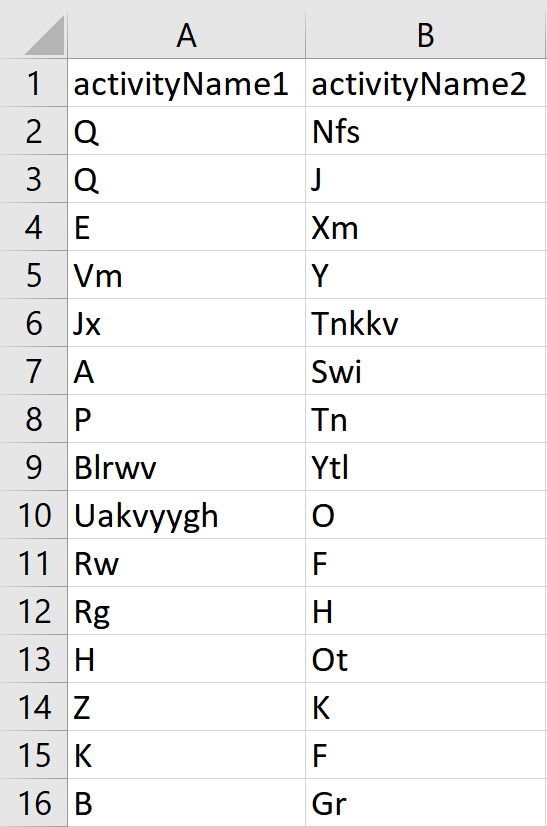
\includegraphics[scale=0.40]{obf.clean.esempio} 
        \caption{Esempio: \emph{clean\_output.csv}}
            \label{fig:obf.clean.es}
    \end{minipage}\hfill
    \begin{minipage}{0.5\textwidth}
        \centering
        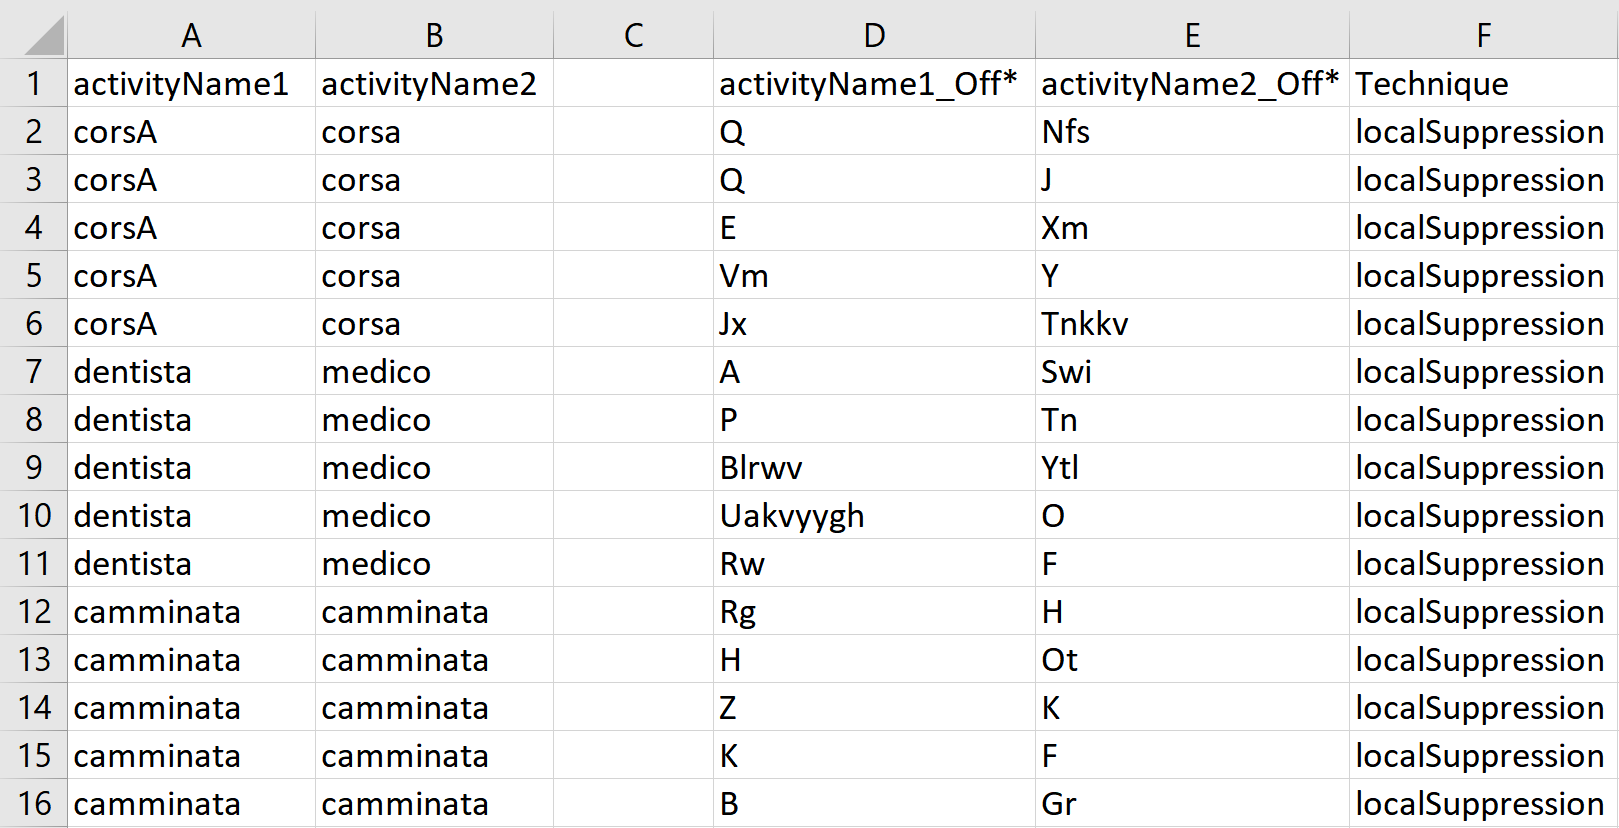
\includegraphics[scale=0.25]{obf.output.esempio} 
        \caption{Esempio: \emph{output.csv}}
            \label{fig:obf.output.es}
    \end{minipage}
\end{figure}


\begin{figure}[H]
	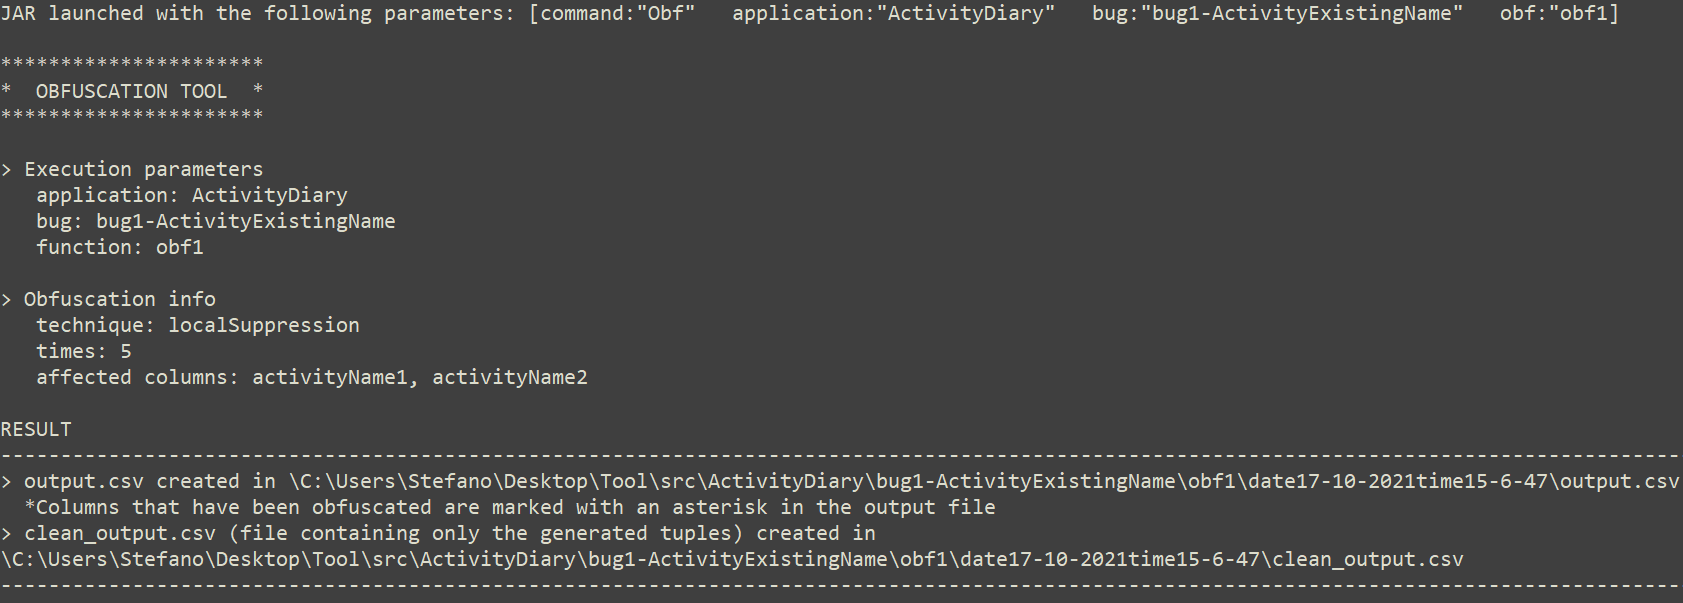
\includegraphics[scale=0.45]{log.esempio}
	\centering
	\caption{Esempio: \emph{log.txt}}
    \label{fig:loges}
\end{figure}

\noindent Per ogni esecuzione della funzionalità viene creata una cartella contenente i file prodotti appena discussi. Il nome della cartella dipende dal momento in cui il tool è stato eseguito e segue un pattern di questo tipo: 'dateDD-MM-YYYYtimeHH-MM-SS'. La cartella viene posizionata all'interno del package di lancio nel percorso  src/\emph{@application}/\emph{@bug}/\emph{@obf}.  In Figura \ref{fig:outdir} vengono mostrate le cartelle create per ogni esecuzione della funzionalità con specifici parametri .  

\begin{figure}[H]
	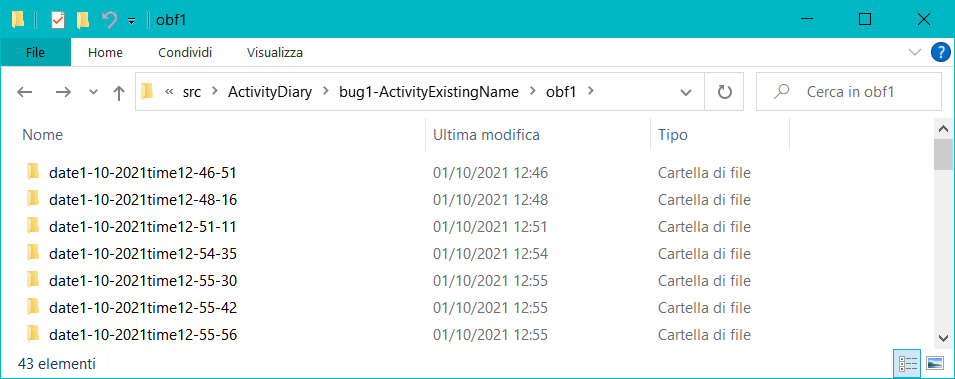
\includegraphics[scale=0.50]{output.directory}
	\centering
	\caption{Esempio: cartelle di esecuzione}
    \label{fig:outdir}
    \emph{Cartelle create per le esecuzioni della funzionalità con parametri in input @application="ActivityDiary", @bug="bug1-ActivityExistingName", @obf="obf1"}
\end{figure}


\newpage %TEMPORANEO
\subsection{Automatizzazione dei test}
\label{sub:AutomatizzaTest}
La funzionalità 'Automatizzazione dei test' si occupa dell'automazione dei test rispondendo al requisito funzionale \emph{Fu.2}. Specificatamente la funzionalità permette di eseguire automaticamente test parametrici su applicazioni Android e, per ogni test, di catturare il risultato e verificare se il bug atteso è stato riprodotto. Inoltre viene offerta la possibilità di salvare uno screenshot o uno screen record per ogni esecuzione del test parametrizzato.


\subsection*{Architettura della soluzione}
\begin{figure}[H]
	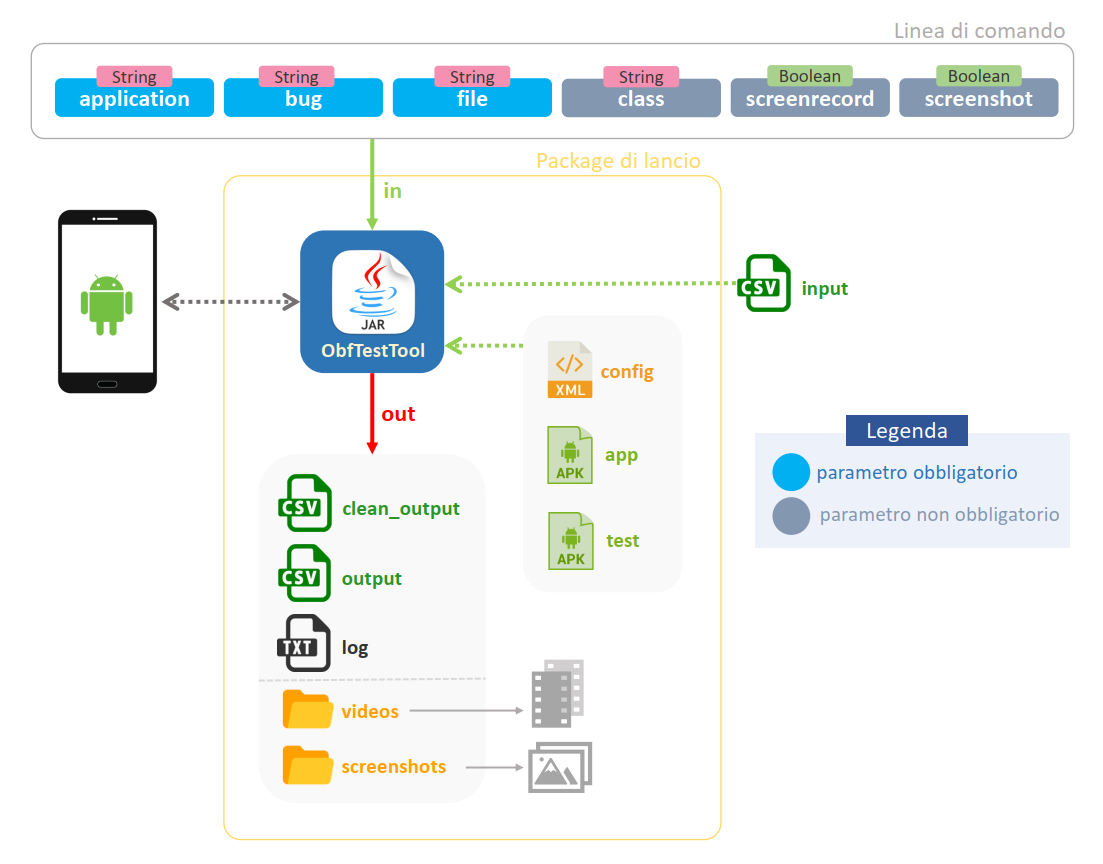
\includegraphics[scale=0.60]{automation.architettura}
	\centering
	\caption{Architettura della soluzione}%\footnote{Immagine realizzata da A. Belisario}
    \label{fig:autarch}
\end{figure}
Come illustrato in Figura \ref{fig:autarch}, il tool, nell'eseguire la funzionalità considerata, richiede obbligatoriamente alcuni parametri:
\begin{itemize} [nosep]
\item \textbf{\emph{@application}} id dell'applicazione \emph{[dominio: String]}
\item \textbf{\emph{@bug}} id del bug \emph{[dominio: String]}
\item \textbf{\emph{@file}} path del file csv contenente i parametri con cui lanciare i test (deve essere strutturato nello stesso modo del file di input dei dati trattato nella Sezione \ref{filediinputdeidati})  \emph{[dominio: String]} \newline
\end{itemize}
\noindent L'esecuzione della funzionalità 'Automatizzazione dei test' può essere personalizzata specificando altri parametri non obbligatori:
\begin{itemize} [nosep]
\item \textbf{\emph{@class}} pacchetto interno in cui si trova la classe di test con aggiunta del nome della classe di test (vedere Appendice A - Generazione degli APK - 1.Creazione della classe di test - Posizione della classe di test) \emph{[dominio: String]} \newline
\textcolor{gray}{valore di default} nome della classe lanciabile del file app.apk + "Test" 
\item \textbf{\emph{@screenrecord}} valore booleano che indica se si vuole utilizzare la funzionalità di salvataggio di uno screen record per ogni esecuzione del test parametrizzato  \emph{[dominio: Boolean (true, false)]} \newline
\textcolor{gray}{valore di default} false
\item \textbf{\emph{@screenshot}} valore booleano che indica se si vuole utilizzare la funzionalità di salvataggio di uno screenshot per ogni esecuzione del test parametrizzato  \emph{[dominio: Boolean (true, false)]} \newline
\textcolor{gray}{valore di default} false
\end{itemize}
\bigskip
\noindent Grazie ai parametri passati, lo strumento è in grado di leggere dal package di lancio (Sezione \ref{sub:strpackage}) alcune informazioni essenziali all'esecuzione della funzionalità:
\begin{itemize} [nosep]

\item [$\blacksquare$]\textbf{app.apk} \newline
Ottiene il file APK dell'applicazione da testare cercando un file con estensione 'apk' all'interno del package di lancio nel percorso  src/\emph{@application}.
\item [$\blacksquare$]\textbf{test.apk} \newline
Ottiene il file APK di test dell'applicazione da testare cercando un file con estensione 'apk' all'interno del package di lancio nel percorso  src/\emph{@application}/\emph{@bug}.
\item [$\blacksquare$]\textbf{tipo di bug atteso} \newline
Ottiene il tipo di bug atteso leggendo il file di configurazione posizionato nel percorso src/config.xml. In particolar modo, effettuando il parsing del file xml, è in grado di ottenere il tipo di bug del bug con id \emph{@bug} dell'applicazione con id \emph{@application}.
\item [$\blacksquare$]\textbf{id dell'emulatore } \newline
Ottiene l'id dell'emlutaore su cui lanciare i test leggendo il file di configurazione posizionato nel percorso src/config.xml. In particolar modo, effettuando il parsing del file xml, è in grado di ottenere l'id dell'emulatore associato al bug con id \emph{@bug} dell'applicazione con id \emph{@application}.
\item [$\blacksquare$]\textbf{nome dell'AVD} \newline
Ottiene il nome dell'AVD su cui lanciare i test leggendo il file di configurazione posizionato nel percorso src/config.xml. In particolar modo, effettuando il parsing del file xml, è in grado di ottenere il nome dell'AVD avente come id l'identificativo trovato al punto precedente.
\end{itemize}
\medskip 
\noindent A questo punto il tool è in possesso di tutte le informazioni necessarie ad eseguire la funzionalità e può lanciare i test parametrici sull'emulatore. 
\smallskip  \newline 

\noindent L'esecuzione della funzionalità, nel caso in cui vada a buon fine, porta alla produzione dei seguenti file:

\begin{tcolorbox}[colback=white, colframe=lightgray]
	 
\includegraphics[height=1cm]{icona.clean} \newline
Il file \emph{clean\_output.csv} è semplicemente una copia del file in input (percorso \emph{@file}) contenente i parametri con cui lanciare i test. Il suo mantenimento in memoria permette in qualsiasi momento di poter rieseguire la funzionalità con gli stessi parametri di test.
\end{tcolorbox}

\begin{tcolorbox}[colback=white, colframe=lightgray]
	 
\includegraphics[height=1cm]{icona.output} \newline
Il file \emph{output.csv} può essere considerato il file riepilogativo dell'esecuzione della funzionalità in quanto contiene i parametri del test, il risultato di ogni test (trattato nel Paragrafo 'Risultato del test') e l'esito della riproduzione del bug atteso (trattato nel Paragrafo 'Logica per la verifica della riproduzione del bug'). Il file ha una struttura del tipo [Val1; Val2; ...; Valn; \textcolor{gray}{NULL}; TestResult;Info;BugReproduction;]. In Figura \ref{fig:aut.output.es} viene mostrato un esempio del file prodotto. 
\end{tcolorbox}

\begin{tcolorbox}[colback=white, colframe=lightgray]
	 
\includegraphics[height=1cm]{icona.log} \newline
Il file \emph{log.txt} contiene semplicemente l'output generato dall'esecuzione della funzionalità sul Command Prompt. Inoltre nel documento vengono salvati come coppie chiave-valore i parametri con cui il tool è stato lanciato. In Figura \ref{fig:aut.log.es} viene mostrato un esempio del file prodotto.  
\end{tcolorbox}


\begin{figure}[H]
	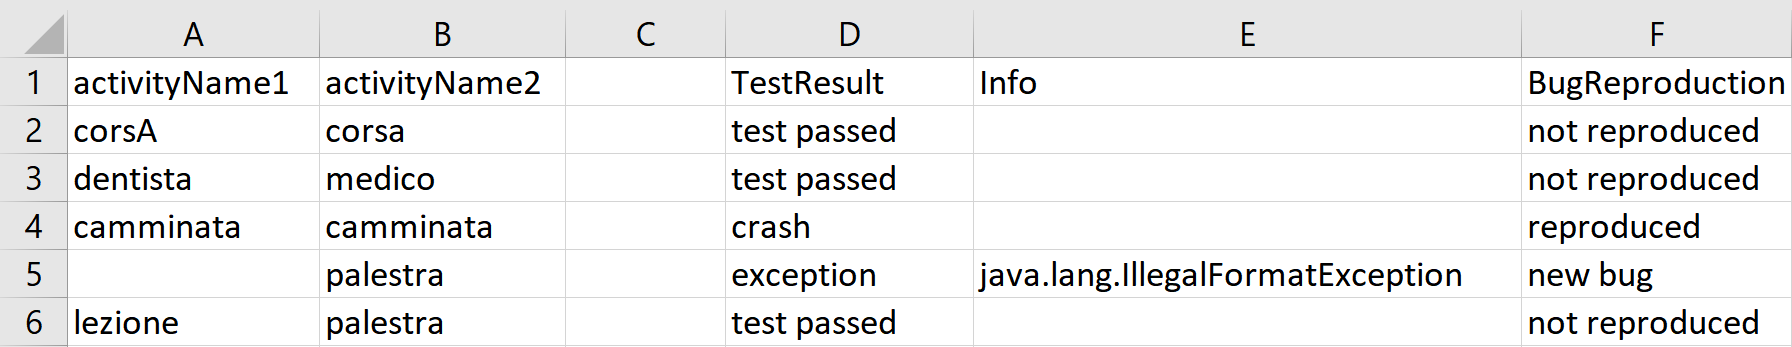
\includegraphics[scale=0.30]{aut.output.esempio}
	\centering
	\caption{Esempio: \emph{output.csv}}
    \label{fig:aut.output.es}
\end{figure}

\begin{figure}[H]
	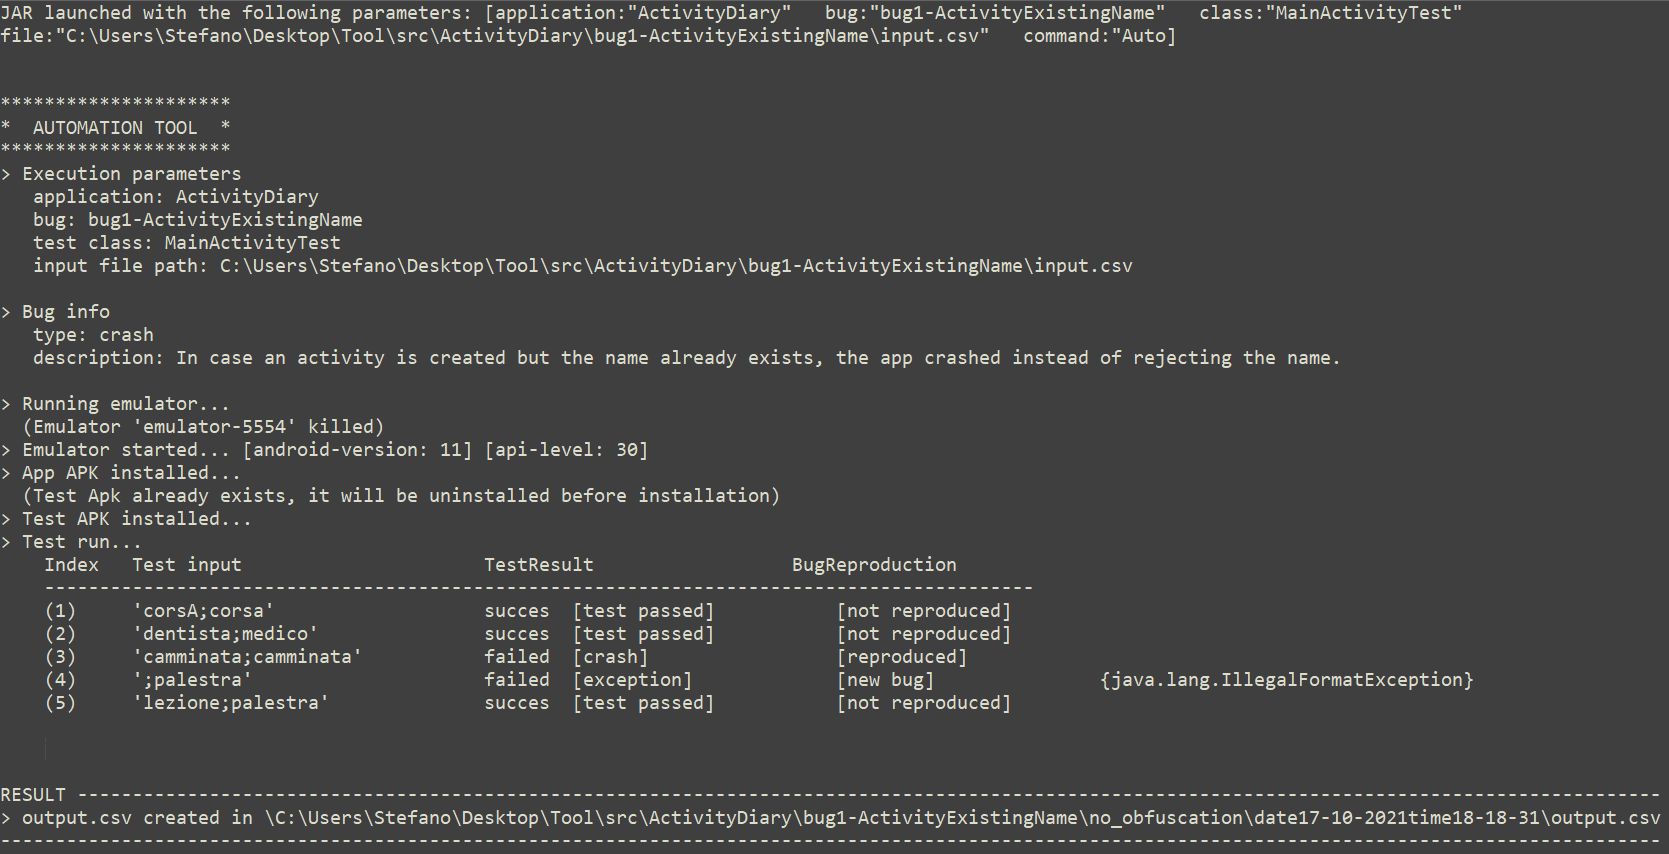
\includegraphics[scale=0.45]{log.aut.esempio}
	\centering
	\caption{Esempio: \emph{log.txt}}
    \label{fig:aut.log.es}
\end{figure}

\noindent Inoltre, in base ai parametri con cui la funzionalità viene lanciato, potrebbero essere prodotti anche:
\begin{tcolorbox}[colback=white, colframe=lightgray]
	 
\includegraphics[height=1cm]{icona.videos} \newline
La cartella videos contiene la registrazione dello schermo (in formato mp4) per ogni test lanciato. La funzionalità viene trattata nel dettaglio nella Sezione \ref{gsr}.
\end{tcolorbox}

\begin{tcolorbox}[colback=white, colframe=lightgray]
	 
\includegraphics[height=1cm]{icona.screenshots} \newline
La cartella screenshots contiene un'istantanea dello schermo (in formato png) per ogni test lanciato. La funzionalità viene trattata nel dettaglio nella Sezione \ref{gss}.
\end{tcolorbox}

\noindent Per ogni esecuzione della funzionalità viene creata una cartella contenente i file prodotti appena discussi. Il nome della cartella dipende dal momento in cui il tool è stato eseguito e segue un pattern di questo tipo: 'dateDD-MM-YYYYtimeHH-MM-SS'. La cartella viene posizionata all'interno del package di lancio nel percorso  src/\emph{@application}/no\_obfuscation.   
%PROVVISORIO
\newpage

\subsection*{Risultato del test}
L'esecuzione di ogni test parametrico può terminare nei seguenti modi:
\begin{itemize}[nosep]
\item [$\blacksquare$] \textbf{crash} \newline
L'applicazione termina in crash senza sollevare nessuna eccezione. 
\item [$\blacksquare$] \textbf{exception} \newline
L'esecuzione del test termina con il sollevamento di un'eccezione non gestita. Il tool è in grado di catturare il tipo di eccezione.
\item [$\blacksquare$] \textbf{test passed} \newline
L'esecuzione del test termina con successo: non è stata sollevata nessuna eccezione, l'applicazione non è terminata in crash e, nel caso in cui il caso di test la preveda, l'asserzione è stata verificata.
\item [$\blacksquare$] \textbf{test not passed} \newline
L'esecuzione del test fallisce perchè l'asserzione non è stata verificata (non perchè l'applicazione è terminata con un crash o è stata sollevata un'eccezione). Questo tipo risultato quindi può verificarsi solo nel caso in cui il caso di test preveda un'asserzione.
\end{itemize}


\subsection*{Logica per la verifica della riproduzione del bug} \label{valbugatt}
Lo strumento, come analizzato, è in grado di verificare se il bug atteso è stato riprodotto. Nel file di configurazione generale \emph{config.xml} , come illustrato nella Sezione \ref{fileconfigfileinput}, per ogni bug può essere specificato il tipo di bug atteso, con la possibilità di scegliere tra uno dei seguenti valori:
\begin{itemize} [nosep]
\item [$\blacksquare$] \textbf{assertion} \newline
Il bug atteso si manifesta quando una o più asserzioni non vengono verificate e quindi se il risultato del test è \emph{test not passed}.
\item  [$\blacksquare$] \textbf{crash} \newline
Il bug atteso si manifesta quando l'applicazione termina in crash e quindi se il risultato del test è \emph{crash}.
\item  [$\blacksquare$] \textbf{exception} \newline
Il bug atteso si manifesta quando l'applicazione solleva un'eccezione, e quindi se il risultato del test è \emph{exception}, e il tipo di eccezione sollevato corrisponde con il tipo di eccezione atteso. Infatti, in questo caso, è obbligatorio aggiungere una colonna chiamata 'expectedException' sia nel file di configurazione che nel file di input, che abbia come valore il tipo di accezione attesa. La Figura \ref{fig:exc.es} potrebbe essere utile ad una migliore comprensione della situazione appena illustrata.
\item [$\blacksquare$]  \textbf{NS} \newline
Il bug atteso non può essere classificato in nessuno dei casi precedenti. In questa situazione risulta utile utilizzare le funzionalità di salvataggio degli screenhots e degli screen record ed effettuare la verifica manualmente.
\end{itemize}

\begin{figure}[H]
	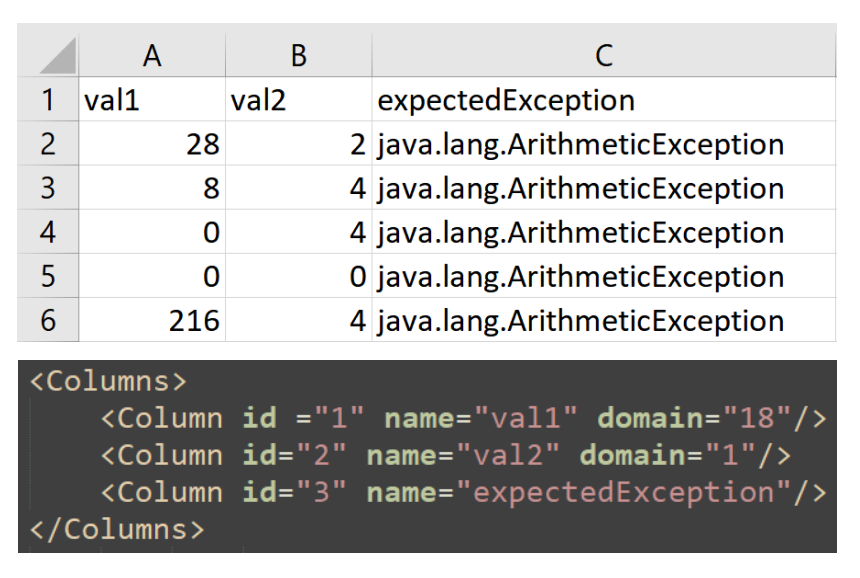
\includegraphics[scale=0.45]{exception.esempio}
	\centering
	\caption{Esempio: configurazione bug di tipo \emph{exception}}
    \label{fig:exc.es}
\end{figure}
\noindent
La verifica della riproduzione del bug atteso (campo 'BugReproduction' nel file di output \emph{output.csv}) può terminare con uno dei seguenti valori:
\begin{itemize} [nosep]
\item [$\blacksquare$] \textbf{reproduced} \newline
Il bug atteso è stato riprodotto, in base alla logica appena esposta.
\item [$\blacksquare$] \textbf{not reproduced}\newline
Il bug atteso non è stato riprodotto, in base alla logica appena esposta, e non si sono presentati altri bug.
\item [$\blacksquare$] \textbf{new bug}\newline
Il bug atteso non è stato riprodotto, in base alla logica appena esposta, ma si è verificato un nuovo bug. Questo caso può verificarsi nelle seguenti situazioni:
\begin{itemize}
\item Il bug atteso è di tipo 'assertion', ma è stata sollevata un'eccezione 
\item Il bug atteso è di tipo 'assertion', ma l'applicazione è terminata con un crash
\item Il bug atteso è di tipo 'exception', ma l'applicazione è terminata con un crash
\item Il bug atteso è di tipo 'crash', ma è stata sollevata un'eccezione
\end{itemize}
\end{itemize}

\newpage %TEMPORANEO
\noindent La logica per la verifica della riproduzione del bug può essere sintetizzata nella tabella illustrata in Figura \ref{fig:logbug}, che considera tutte le possibili combinazioni del caso.

\begin{figure}[H]
	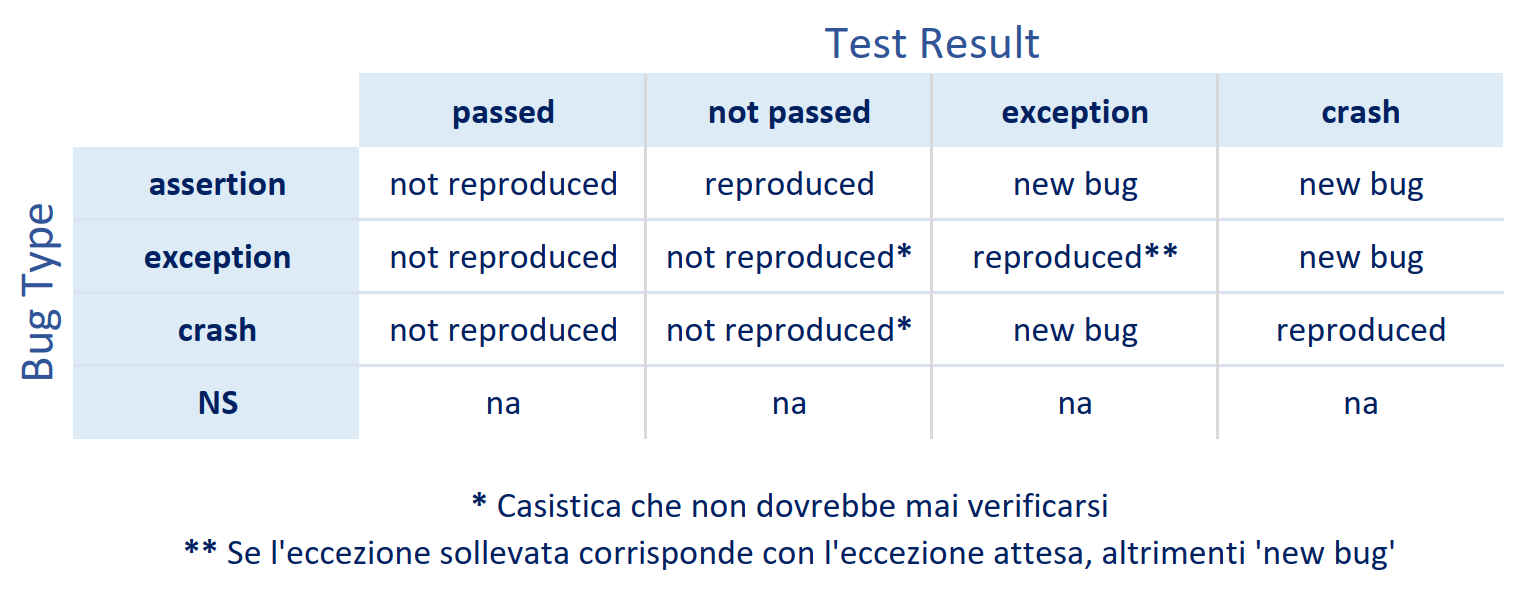
\includegraphics[scale=0.45]{logica.riproduzione.bug}
	\centering
	\caption{Logica per la verifica della riproduzione del bug}
    \label{fig:logbug}
\end{figure}

\noindent Nella tabella sono state inserite anche della casistiche che non dovrebbero idealmente mai verificarsi , infatti:
\begin{itemize}[nosep]
\item [$\blacksquare$]caso \textbf{BugType = 'exception', TestResult = "not passed"} \newline
Nel caso di test che dovrebbe sollevare un'eccezione, non ha senso inserire un'asserzione (il risultato del test  'not passed' si verifica solo quando è presente un'asserzione e questa non è verificata)
\item [$\blacksquare$]caso \textbf{BugType = 'crash', TestResult = "not passed"} \newline
Nel caso di test che dovrebbe provocare un bug dell'applicazione, non ha senso inserire un'asserzione (il risultato del test  'not passed' si verifica solo quando è presente un'asserzione e questa non è verificata)
\end{itemize}


\newpage %TEMPORANEO
\subsection{Offuscamento dei dati e automatizzazione dei test}
La funzionalità 'Offuscamento dei dati e automatizzazione dei test' permette il raggiungimento dell'obiettivo principale dello stage rispondendo al requisito funzionale \emph{Fu.3}. La funzionalità permette di eseguire automaticamente test parametrici utilizzando in input le tuple offuscate ottenute applicando le tecniche di offuscamento sui dati originali che provocano il bug. In questo modo lo strumento è in grado di verificare, per ogni tupla offuscata, se il bug atteso (provocato dalla tupla non offuscata) è stato riprodotto. 

\subsection*{Architettura della soluzione}
\begin{figure}[H]
	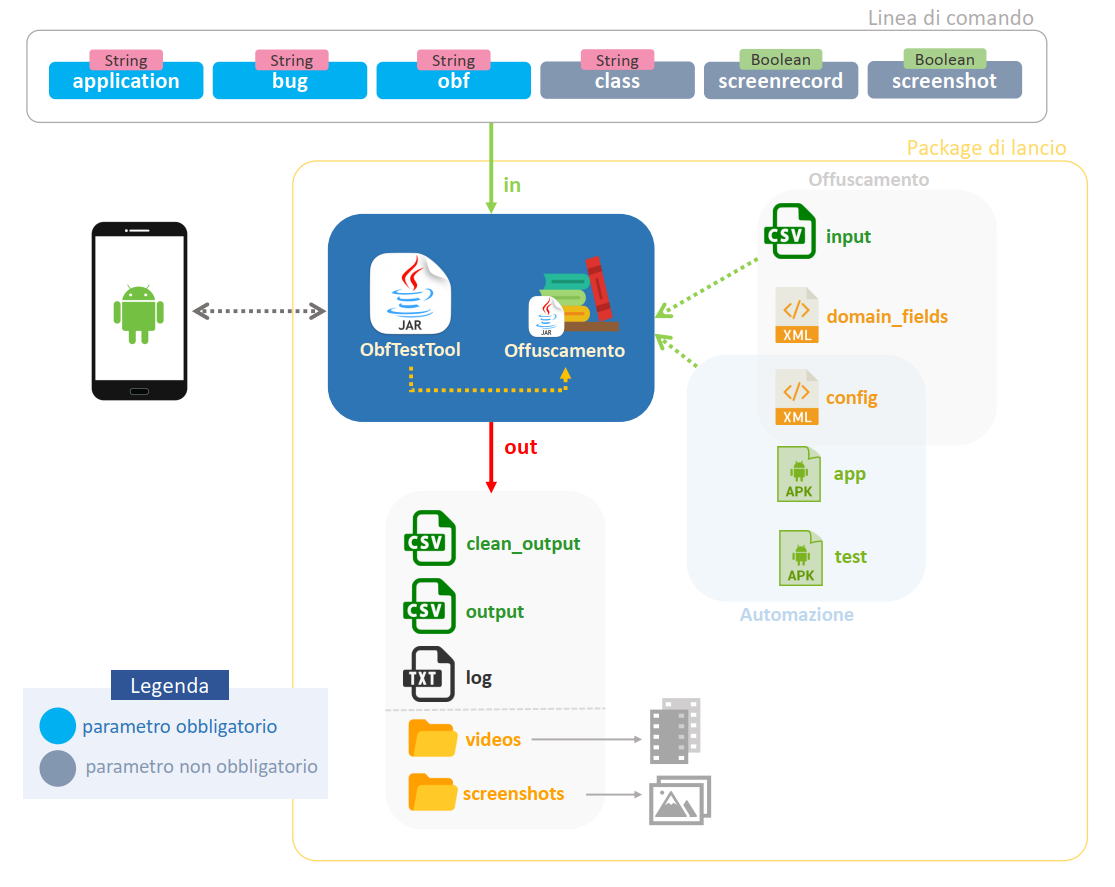
\includegraphics[scale=0.60]{obfuscation.automation.architettura}
	\centering
	\caption{Architettura della soluzione}%\footnote{Immagine realizzata da A. Belisario}
    \label{fig:obfautarch}
\end{figure}

Come illustrato in Figura \ref{fig:obfautarch}, il tool, nell'eseguire la funzionalità considerata, richiede obbligatoriamente alcuni parametri:
\begin{itemize} [nosep]
\item \textbf{\emph{@application}} id dell'applicazione \emph{[dominio: String]}
\item \textbf{\emph{@bug}} id del bug \emph{[dominio: String]}
\item \textbf{\emph{@obf}} id della funzione di offuscamento \emph{[dominio: String]}
\end{itemize}
%TEMPORANEO
\newpage
\noindent L'esecuzione della funzionalità 'Offuscamento dei dati e automatizzazione dei test' può essere personalizzata specificando altri parametri non obbligatori:
\begin{itemize} [nosep]
\item \textbf{\emph{@class}} pacchetto interno in cui si trova la classe di test con aggiunta del nome della classe di test (vedere Appendice A - Generazione degli APK - 1.Creazione della classe di test - Posizione della classe di test) \emph{[dominio: String]} \newline
\textcolor{gray}{valore di default} nome della classe lanciabile del file app.apk + "Test" 
\item \textbf{\emph{@screenrecord}} valore booleano che indica se si vuole utilizzare la funzionalità di salvataggio di uno screen record per ogni esecuzione del test parametrizzato  \emph{[dominio: Boolean (true, false)]} \newline
\textcolor{gray}{valore di default} false
\item \textbf{\emph{@screenshot}} valore booleano che indica se si vuole utilizzare la funzionalità di salvataggio di uno screenshot per ogni esecuzione del test parametrizzato  \emph{[dominio: Boolean (true, false)]} \newline
\textcolor{gray}{valore di default} false
\end{itemize}
\bigskip

\noindent Grazie ai parametri passati, lo strumento è in grado di leggere dal package di lancio (Sezione \ref{sub:strpackage}) le informazioni essenziali all'esecuzione della funzionalità, che sono complessivamente quelle elencate per le singole funzionalità 'Automatizzazione dei test' e 'Offuscamento dei dati' nelle sezioni precedenti.

\noindent A questo punto il tool è in possesso di tutte le informazioni necessarie ad eseguire in sequenza prima l'offuscamento delle tuple e poi l'automazione dei test. L'automazione dei test viene effettuata utilizzando come file di input il file \emph{clean\_output.csv} prodotto dall'offuscamento dei dati.
\bigskip \newline  
\noindent L'esecuzione della funzionalità, nel caso in cui vada a buon fine, porta alla produzione dei seguenti file:
\begin{tcolorbox}[colback=white, colframe=lightgray]
	 
\includegraphics[height=1cm]{icona.clean} \newline
Corrisponde completamente al file \emph{clean\_output.csv} prodotto dalla funzionalità 'Offuscamento dei dati'. 
\end{tcolorbox}

\begin{tcolorbox}[colback=white, colframe=lightgray]
	 
\includegraphics[height=1cm]{icona.output} \newline
Il file \emph{output.csv} può essere considerato il file riepilogativo dell'esecuzione della funzionalità in quanto contiene le tuple originali, le tuple offuscate, la tecnica di offuscamento, il risultato di ogni test e l'esito della riproduzione del bug. Il file ha una struttura del tipo [Val1; Val2; ...; Valn; \textcolor{gray}{NULL}; Val1\_Off; Val2\_Off; ...; Valn\_Off; Technique; \textcolor{gray}{NULL}; TestResult; Info; BugReproduction] in cui, nell'intestazione,  il nome delle colonne che sono state offuscate è seguito da un '*'. In Figura \ref{fig:obfaut.output.es} viene mostrato un esempio del file prodotto.
\end{tcolorbox}


%QUIIIIIIIIIIIIIIIIIIIIII


\begin{tcolorbox}[colback=white, colframe=lightgray]
	 
\includegraphics[height=1cm]{icona.log} \newline
Il file \emph{log.txt} contiene semplicemente l'output generato dall'esecuzione della funzionalità sul Command Prompt. Inoltre nel documento vengono salvati come coppie chiave-valore i parametri con cui il tool è stato lanciato. In Figura \ref{fig:obf.aut.log.es} viene mostrato un esempio del file prodotto.  
\end{tcolorbox}





\begin{figure}[H]
	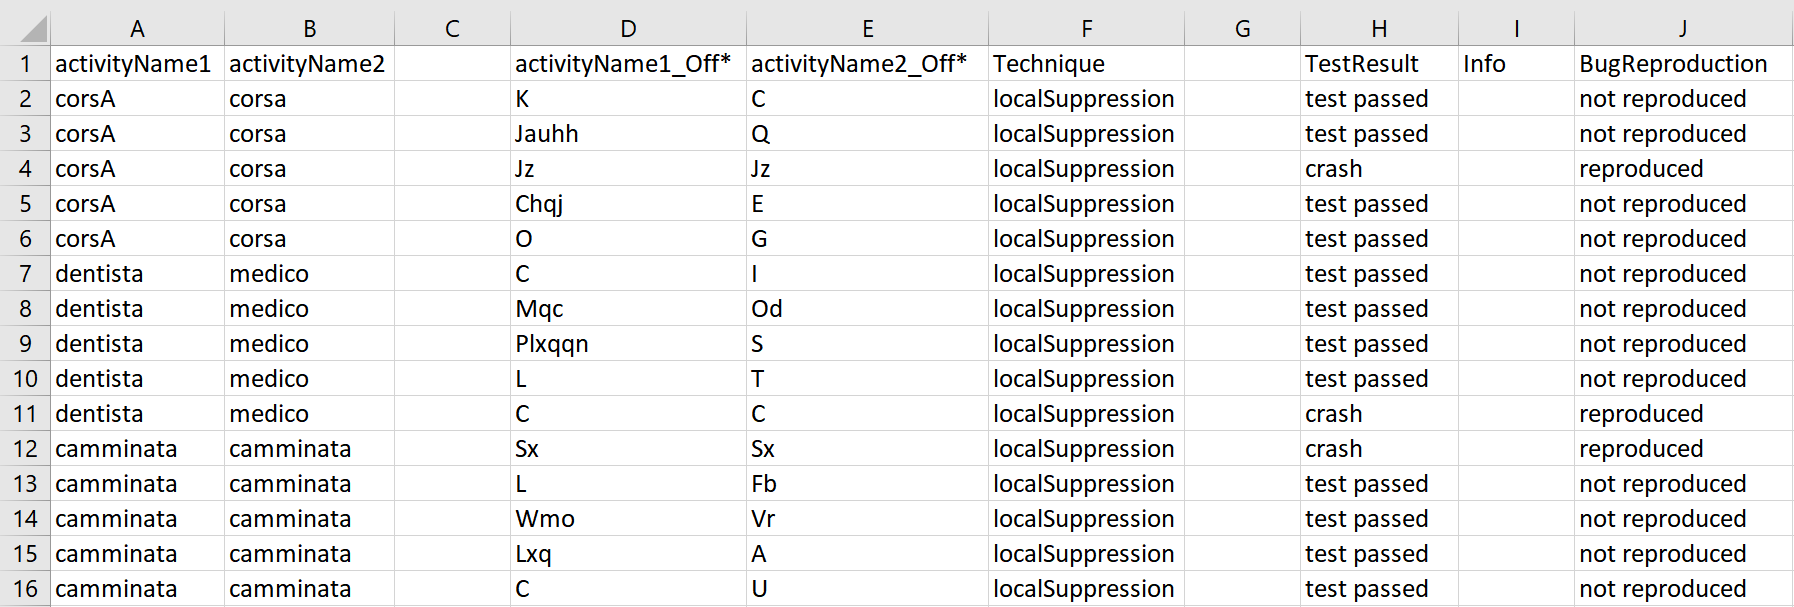
\includegraphics[scale=0.40]{obf.aut.output.esempio}
	\centering
	\caption{Esempio: \emph{output.csv}}
    \label{fig:obfaut.output.es}
\end{figure}

\begin{figure}[H]
	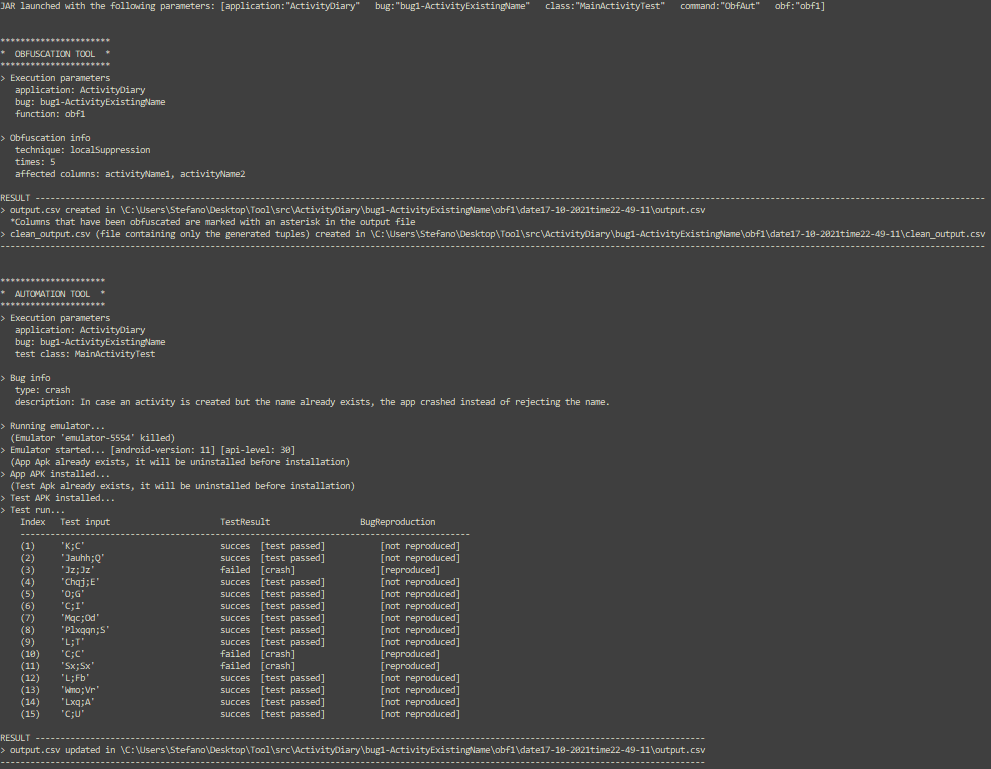
\includegraphics[scale=0.65]{log.obf.aut.esempio}
	\centering
	\caption{Esempio: \emph{log.txt}}
    \label{fig:obf.aut.log.es}
\end{figure}

\noindent Inoltre, in base ai parametri con cui la funzionalità viene lanciata, potrebbero essere prodotti anche:
\begin{tcolorbox}[colback=white, colframe=lightgray]
	 
\includegraphics[height=1cm]{icona.videos} \newline
La cartella videos contiene la registrazione dello schermo (in formato mp4) per ogni test lanciato. La funzionalità viene trattata nel dettaglio nella Sezione \ref{gsr}.
\end{tcolorbox}

\begin{tcolorbox}[colback=white, colframe=lightgray]
	 
\includegraphics[height=1cm]{icona.screenshots} \newline
La cartella screenshots contiene un'istantanea dello schermo (in formato png) per ogni test lanciato. La funzionalità viene trattata nel dettaglio nella Sezione \ref{gss}.
\end{tcolorbox}

\noindent Per ogni esecuzione della funzionalità viene creata una cartella contenente i file prodotti appena discussi. Il nome della cartella dipende dal momento in cui il tool è stato eseguito e segue un pattern di questo tipo: 'dateDD-MM-YYYYtimeHH-MM-SS'. La cartella viene posizionata all'interno del package di lancio nel percorso  src/\emph{@application}/\emph{@bug}/\emph{@obf}.   
%PROVVISORIO
\newpage


